%%%%%%%%%%%%%%%%%%%%%%%%%%%%%%%%%%%%%%%%%
%
% This file defines required packages for building
% and System Initialization.
% Execute before the \begin{document} command.
%
%%%%%%%%%%%%%%%%%%%%%%%%%%%%%%%%%%%%%%%%%

\documentclass[12pt,a4paper]{article}
\usepackage[a4paper, left=2cm, right=2cm, top=2.8cm, bottom=2.3cm]{geometry}
\usepackage[utf8x]{inputenc}
\usepackage{amsmath}
\usepackage{amsfonts}
\usepackage{amssymb}
\usepackage{graphicx}
\usepackage{longtable}
\usepackage{booktabs}
\usepackage{hyperref}
\usepackage{listings}
\usepackage{float}
\usepackage{tikz}
\usepackage[super]{nth}
\usepackage[firstpage]{draftwatermark}
\usepackage{supertabular}
\usepackage{booktabs}

\SetWatermarkLightness{0.9}
\SetWatermarkText{\tikz\node[opacity=0.2]{
	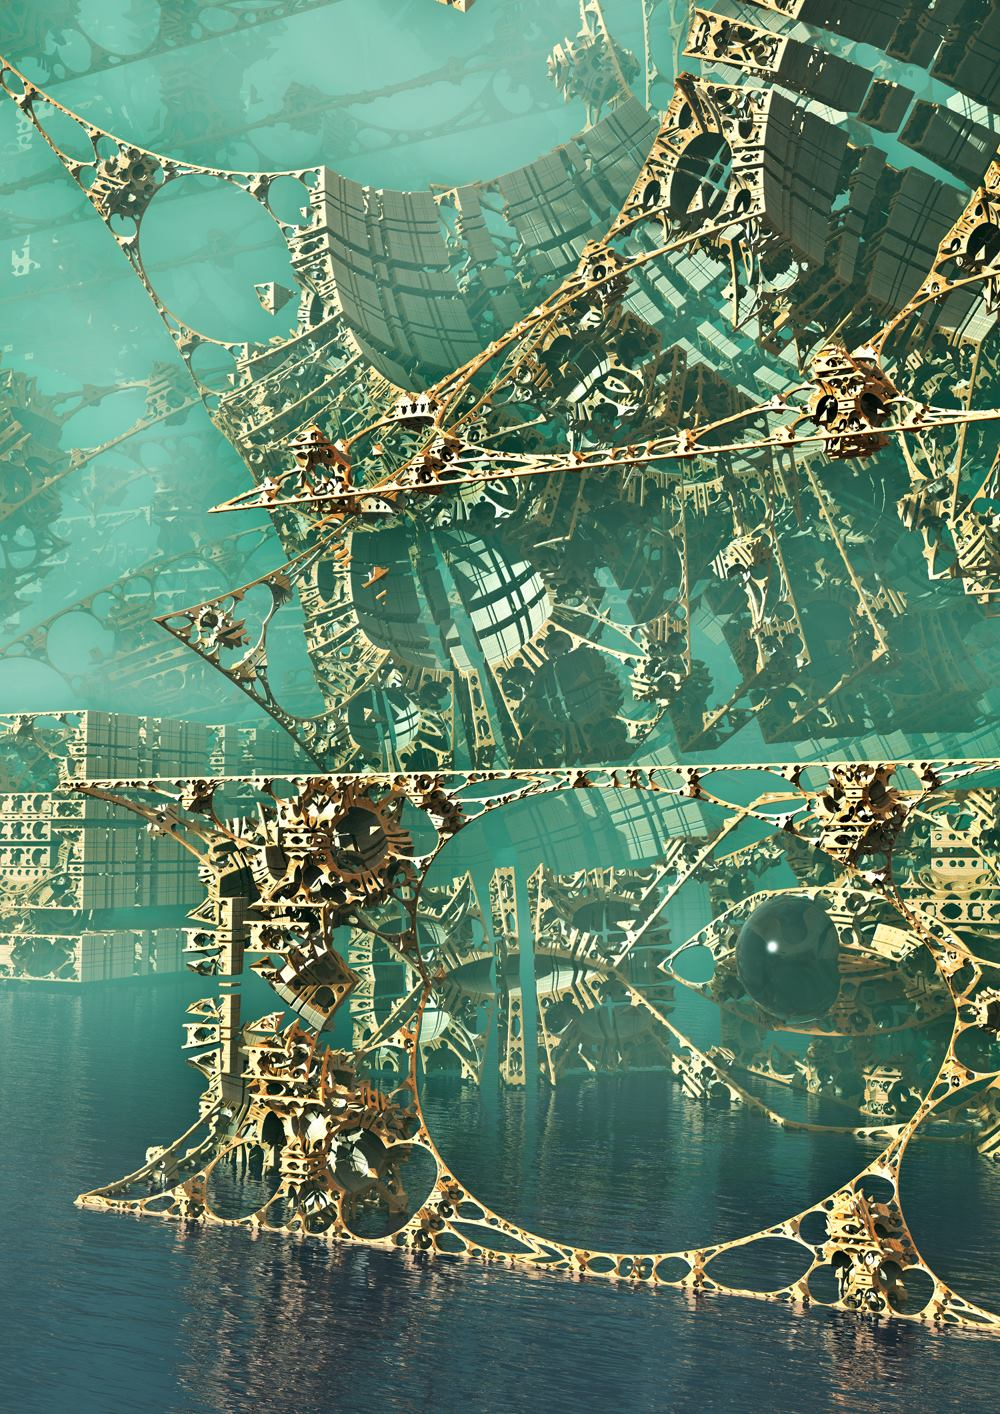
\includegraphics[width=1.0\paperwidth,angle=-45]{img/mandelbulber_background.jpg}};
}

\usepackage[font={footnotesize,it}]{caption}
\usepackage{chngcntr}
\counterwithin{figure}{section}

\usepackage{makeidx}
\usepackage{multicol}

\makeindex

%\usepackage[many]{tcolorbox}
%\newtcolorbox{notebox}[1][]{ 
%	enhanced, 
%	breakable, 
%	pad at break=2mm,
%	left=2mm,
%	right=10mm, 
%	colback=white,
%	colframe=black!50!yellow, 
%	drop fuzzy midday
%	shadow=black!50!yellow, 
%	width={0.95\textwidth}, 
%	frame hidden, 
%	segmentation hidden, 
%	before=\par\vspace*{2mm},
%	after=\par\bigskip, title=#1
%}

\usepackage{fancyvrb}
\DefineVerbatimEnvironment{verbatim}{Verbatim}{xleftmargin=.5in, fontsize=\small, samepage=true}

%\usepackage[default,osfigures,scale=0.95]{opensans} %% open sans text style
\usepackage[sfdefault]{roboto}
\usepackage[T1]{fontenc}
\DeclareMathSizes{13}{12}{11}{10}
\setlength{\parskip}{0.5em}

% Link setup
\hypersetup{
	colorlinks   = true,
	urlcolor     = blue,
	linkcolor    = blue,
	citecolor   = red
}

%deactivated, since too much hassle with setup, see lstlistings instead
% set minted (code formatted) font size 
%\usemintedstyle{emacs}
%\newminted{cpp}{
%	frame=lines,
%	framesep=2mm,
%	baselinestretch=1,
%	fontsize=\footnotesize,
%	% linenos
%}

\lstset{language=C++,
	keywordstyle = \color{blue}\ttfamily,
	stringstyle = \color{red}\ttfamily,
	commentstyle = \color[rgb]{0,0.7,0}\ttfamily,
	morecomment = [l][\color{magenta}]{\#},
	frame=lines,
	framesep=0.5mm,
	basicstyle=\scriptsize\ttfamily
}

\usepackage{titlesec}
\newcommand{\sectionbreak}{\clearpage}

\setlength{\parindent}{0pt} % remove indent on continuous paragraphs

